% Section content template for individual Educative lessons
% This file contains the actual content for a specific section
% Generated from Educative API section content

% Section: Class Diagram for the Amazon Online Shopping System
% Section ID: 6113026015232000
% Section Slug: class-diagram-for-the-amazon-online-shopping-system
% Generated: 2025-12-12T22:45:43.164486

In this lesson, we'll identify and design the classes, abstract classes, and interfaces based on the requirements we previously gathered from the interviewer in our Amazon shopping system.

\subsection{Components of Amazon}\label{GpkLyt7GW5-VOqXXpXFm_}
\\
As mentioned, we should design the Amazon online shopping system using a bottom-up approach.

\subsubsection{Customer}\label{hY4BSdSDGiNBYSYe7VLVs}
\\
The \texttt{Customer} abstract class refers to a user searching for a product on Amazon.
\\
A customer can be one of the following:

\begin{enumerate}
\item
\protect\phantomsection\label{VaSAkpaMwt8js5sMwN5Ps}
Authenticated users
\item
\protect\phantomsection\label{GJ0iVP8hIOde4Awhphjaa}
Guest users
\end{enumerate}
\\
The details of these are given below:

\begin{itemize}
\item
\protect\phantomsection\label{YmWjoALaxBDlevYeVPMlR}
The \texttt{AuthenticatedUser} class refers to an individual with a registered Amazon account.
\item
\protect\phantomsection\label{OWMulwZvkY6Xi-6zUZhge}
The \texttt{Guest} class refers to an individual without an account who can only search for and view the products on the Amazon website. However, they need to register for an account on Amazon to place an order.
\end{itemize}
\\
The class diagram of all these is provided below:

\begin{figure}[htbp]
 \centering
 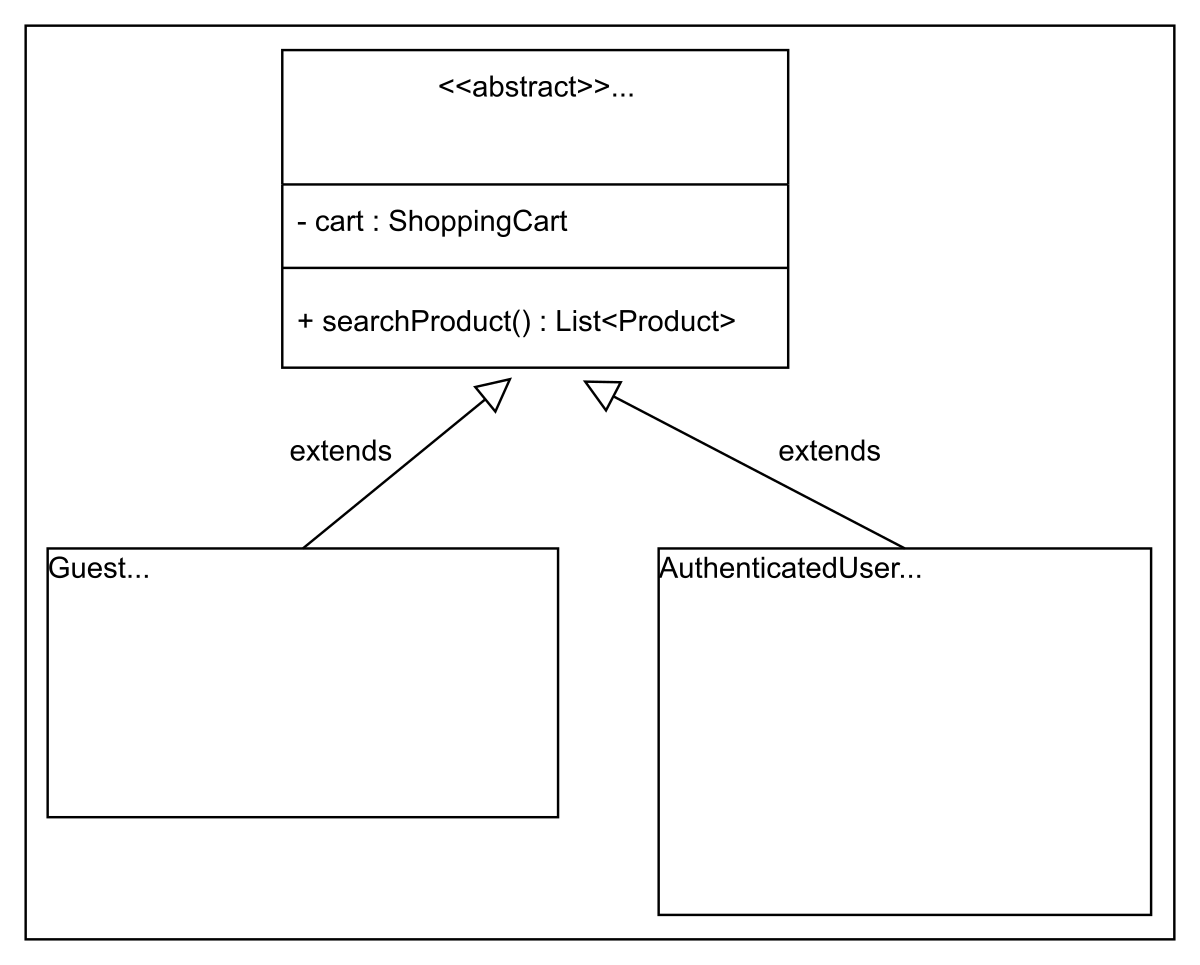
\includegraphics[width=0.5\textwidth]{Images/chapter_19/section_6113026015232000/4942898972721152.png}
 \caption{The class diagram of the Customer class and its child classes}
\end{figure}

\textbf{R1:} A customer can be an authenticated user or a guest. The authenticated user has a registered Amazon online shopping system account, whereas a guest does not.

\subsubsection{Admin}\label{MpzEfCwLoRiYCisXI09z9}
\\
The \texttt{Admin} class refers to an individual with a registered account on Amazon who can add, modify, or delete product categories and block users.

\begin{figure}[htbp]
 \centering
 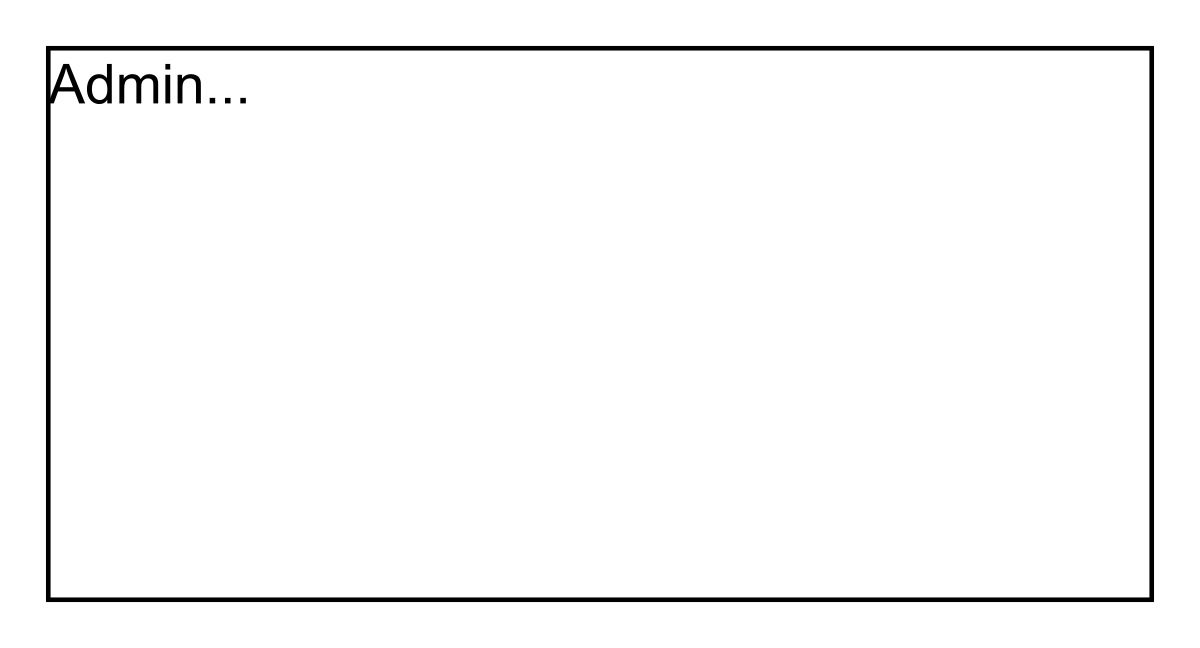
\includegraphics[width=0.5\textwidth]{Images/chapter_19/section_6113026015232000/4625003835162624.png}
 \caption{The class diagram of the Admin class}
\end{figure}

\textbf{R10:} An admin who can add or modify product categories and block users should exist.

\subsubsection{Account}\label{Jn-6-EQNUO_5m2VtDVZA_}
\\
The \texttt{Account} class accesses and showcases the personal details of the authenticated user and the admin, the two types of registered accounts available in the system. Users with an account can add and delete products and product reviews.

\begin{figure}[htbp]
 \centering
 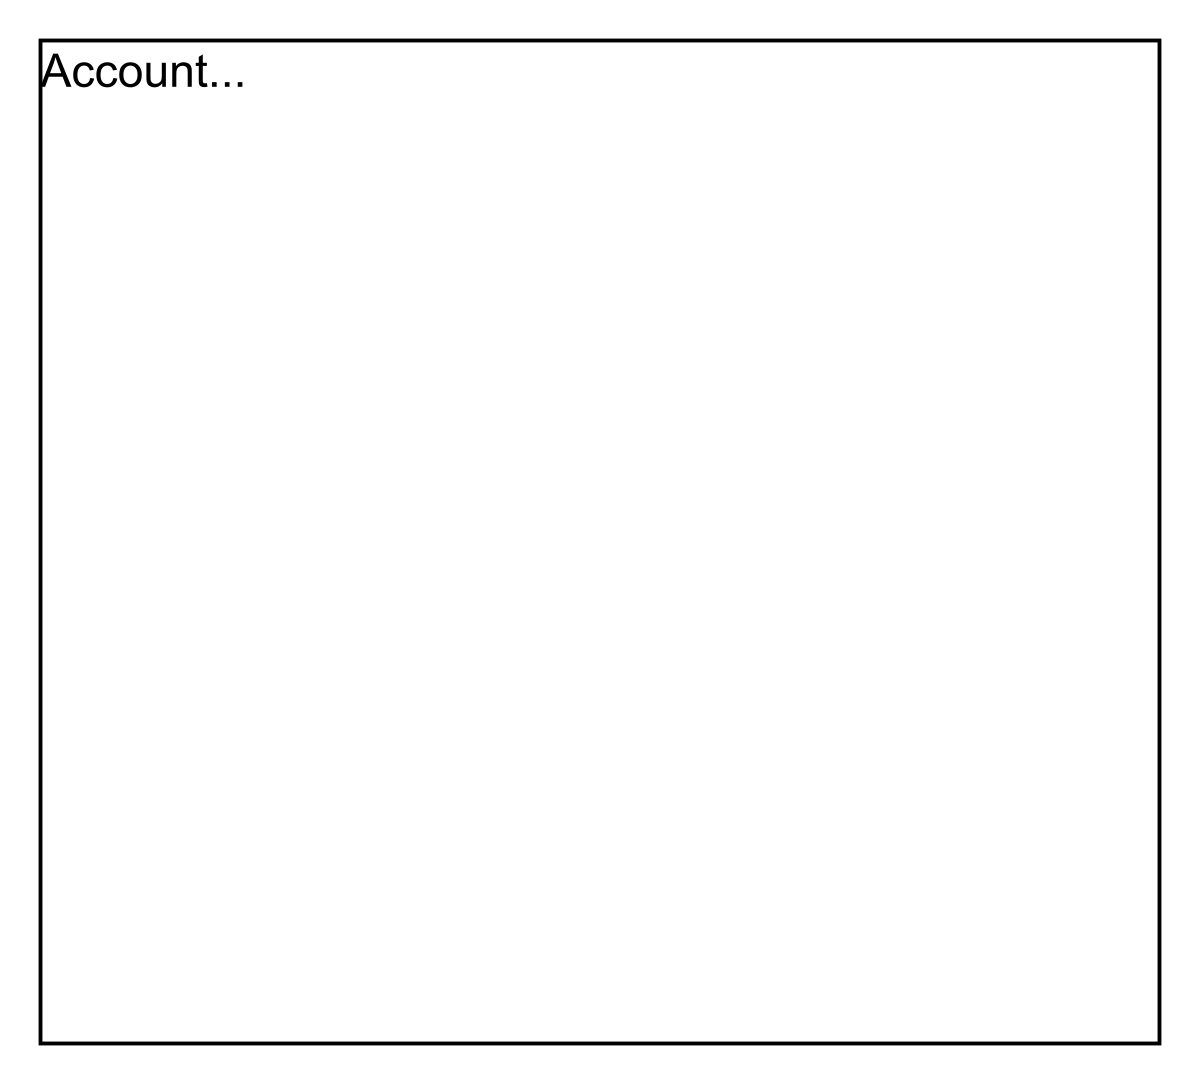
\includegraphics[width=0.5\textwidth]{Images/chapter_19/section_6113026015232000/6172384284246016.png}
 \caption{The class diagram of the Account class}
\end{figure}

\textbf{R1:} A customer can be an authenticated user or a guest. The authenticated user has a registered account on the Amazon online shopping system, whereas a guest doesn't have a registered account.
\\
\textbf{R11:} An account should store personal information such as name, email, password, and other relevant details for admins and authenticated users.

\subsubsection{Product}\label{M7KDM0paH0jNV4ObApEQc}
\\
The \texttt{Product} class contains the details of a particular product on the Amazon shopping store. Each product falls under a specific category on Amazon and can have none, one, or more reviews.

\begin{figure}[htbp]
 \centering
 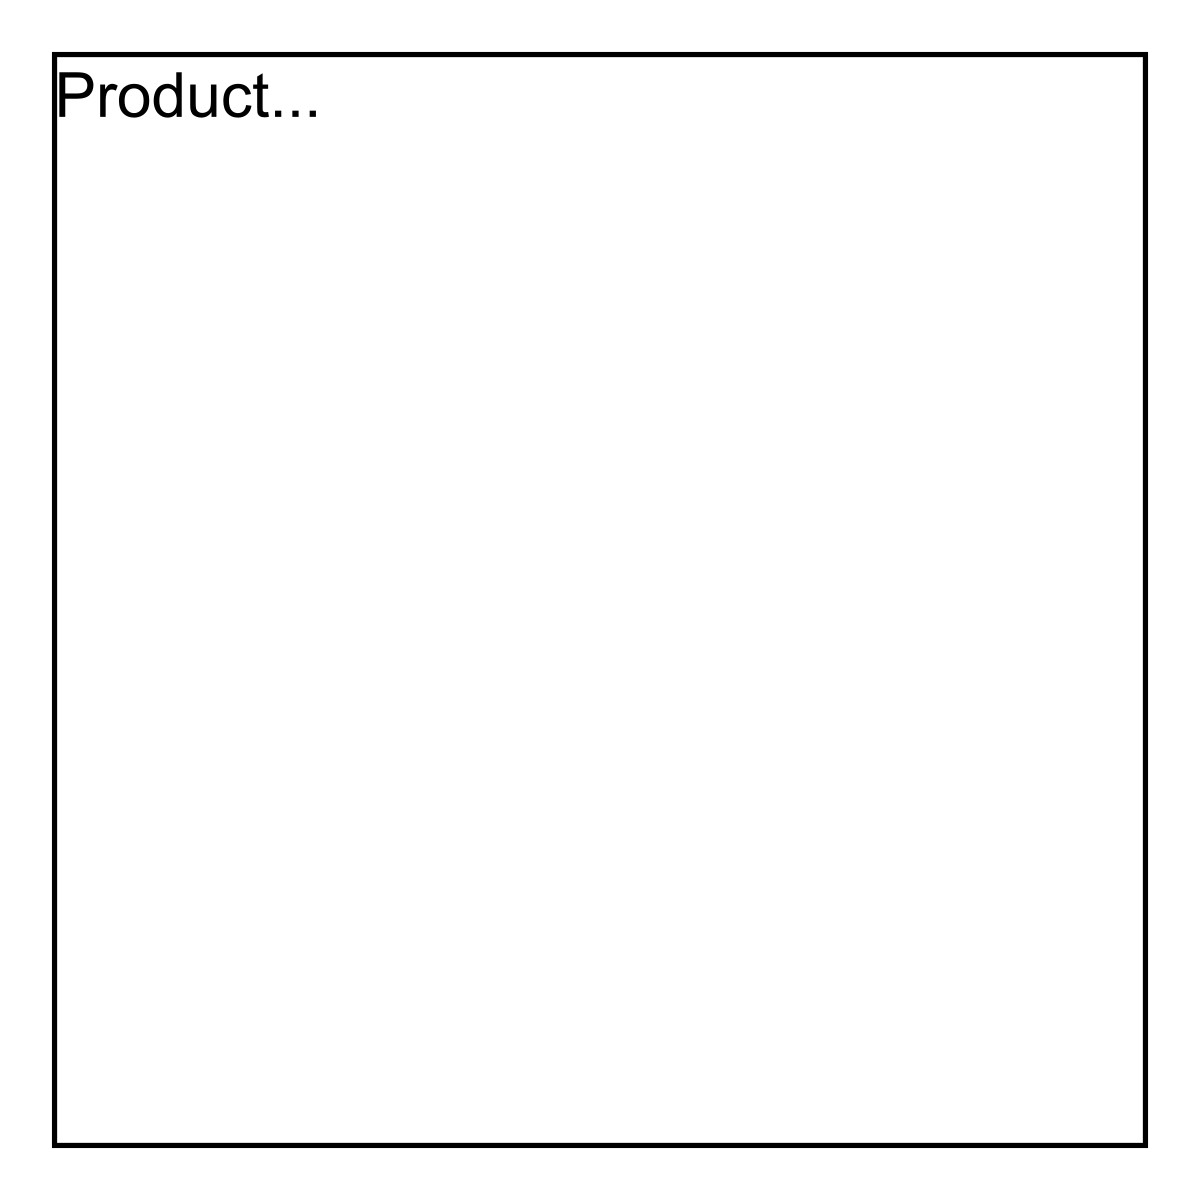
\includegraphics[width=0.5\textwidth]{Images/chapter_19/section_6113026015232000/5495398956138496.png}
 \caption{The class diagram of the Product class}
\end{figure}

\textbf{R3:} A product can have multiple reviews and ratings from multiple customers.

\subsubsection{Product category}\label{DIgbUQpz-CePcFMdbYSCW}
\\
The \texttt{ProductCategory} class contains the names and descriptions of Amazon's various product categories and a reference to the list of products in each category.

\begin{figure}[htbp]
 \centering
 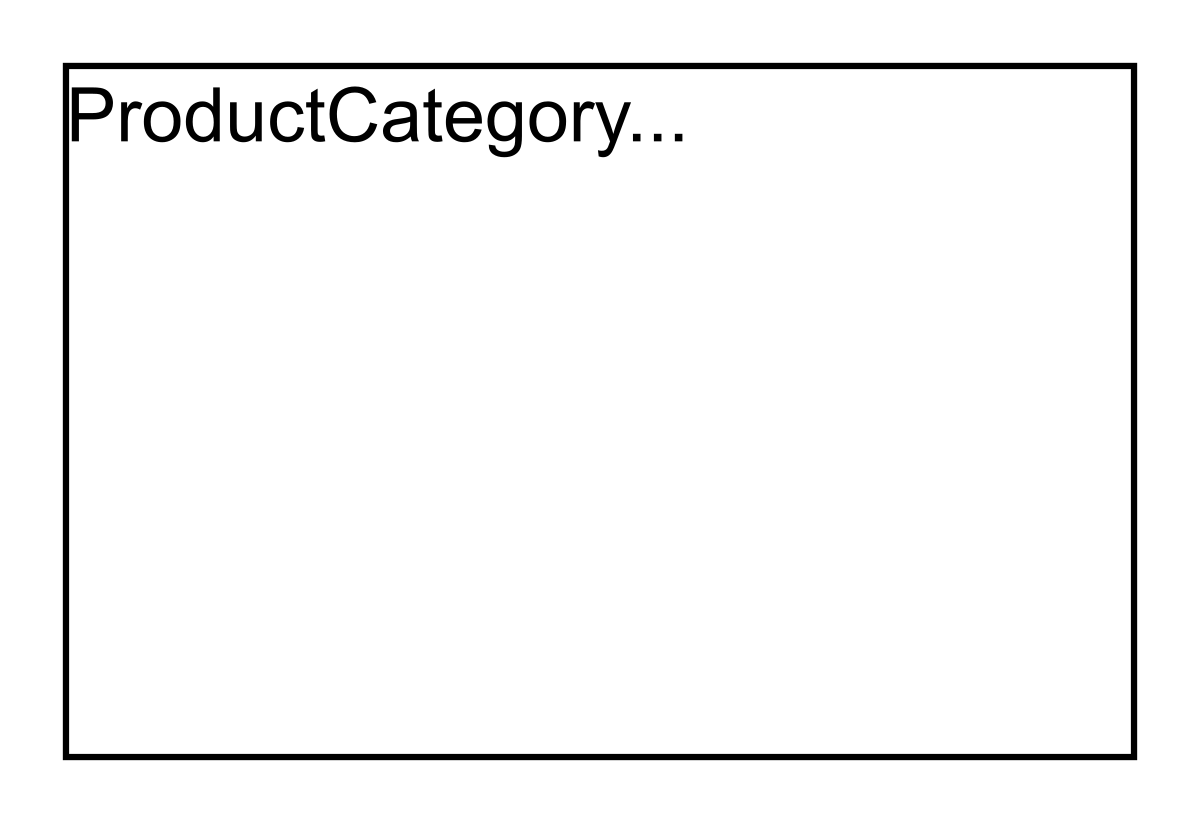
\includegraphics[width=0.5\textwidth]{Images/chapter_19/section_6113026015232000/6591157218705408.png}
 \caption{The class diagram of the ProductCategory class}
\end{figure}

\textbf{R2:} An authenticated user should be able to buy, sell, and search the products via the product name or category. A guest is only able to search for products.

\subsubsection{Product review}\label{QfPsENZs5lCIKTsBiExAm}
\\
The \texttt{ProductReview} class contains the rating and review attributes a registered user can use to add a review about a particular product.

\begin{figure}[htbp]
 \centering
 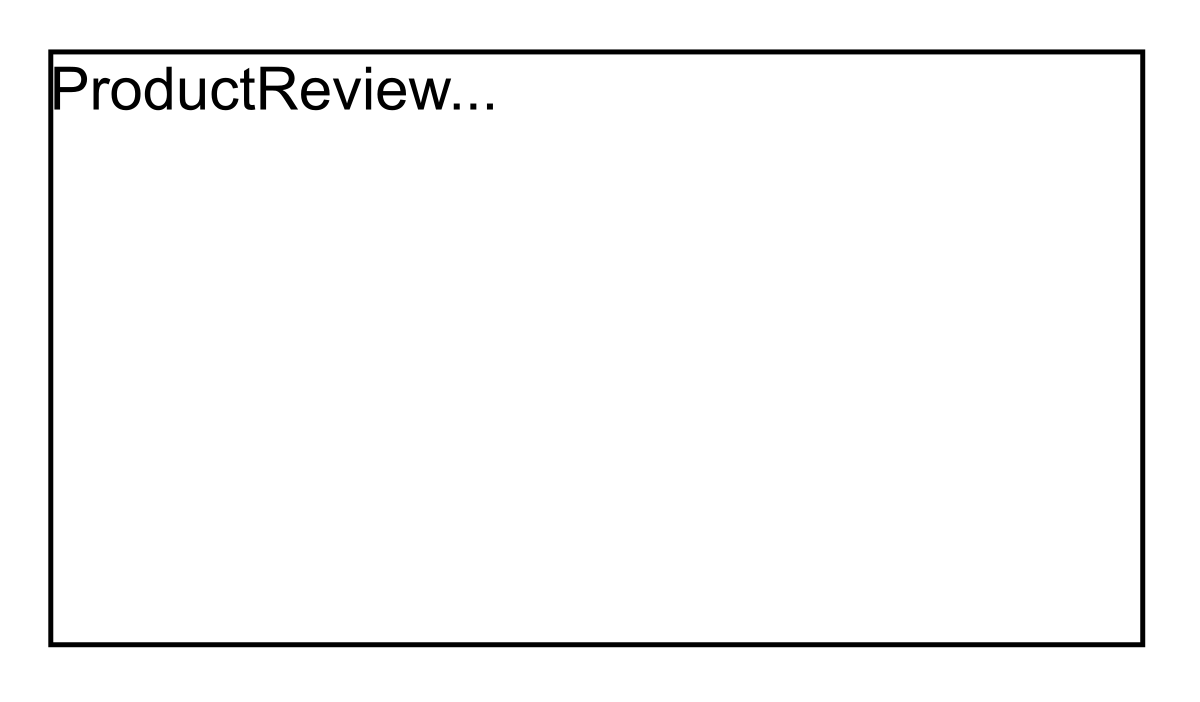
\includegraphics[width=0.5\textwidth]{Images/chapter_19/section_6113026015232000/6597698078507008.png}
 \caption{The class diagram of the ProductReview class}
\end{figure}

\textbf{R3:} A product can have multiple reviews and ratings from multiple customers.

\subsubsection{Search}\label{eMDaZ-zjBY3tIYRHmfjSf-2}
\\
The \texttt{Search} class will be an interface that contains the functionalities relating to searching for products.

\begin{figure}[htbp]
 \centering
 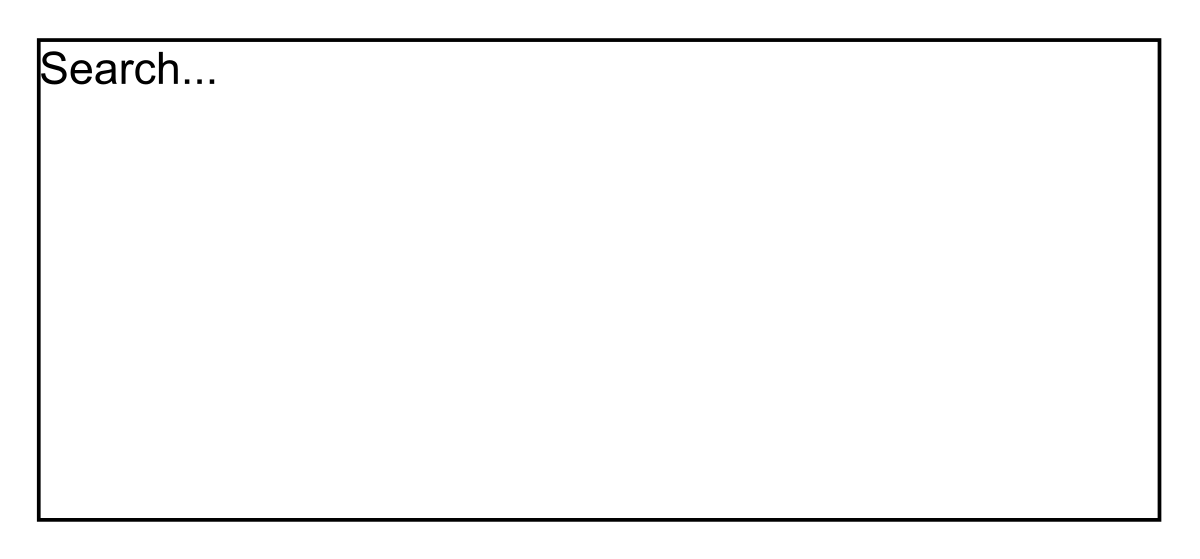
\includegraphics[width=0.5\textwidth]{Images/chapter_19/section_6113026015232000/4732947402719232.png}
 \caption{The class diagram of the Search interface}
\end{figure}

\textbf{R2:} An authenticated user should be able to buy, sell, and search the products via the product name or category. A guest is only able to search for products.

\subsubsection{Cart item}\label{cfrHtdpcrmyod2m_HGKVm}
\\
The \texttt{CartItem} class refers to the items in the shopping cart. It will have price and quantity attributes, which can be modified using the \texttt{updateQuantity()} function.

\begin{figure}[htbp]
 \centering
 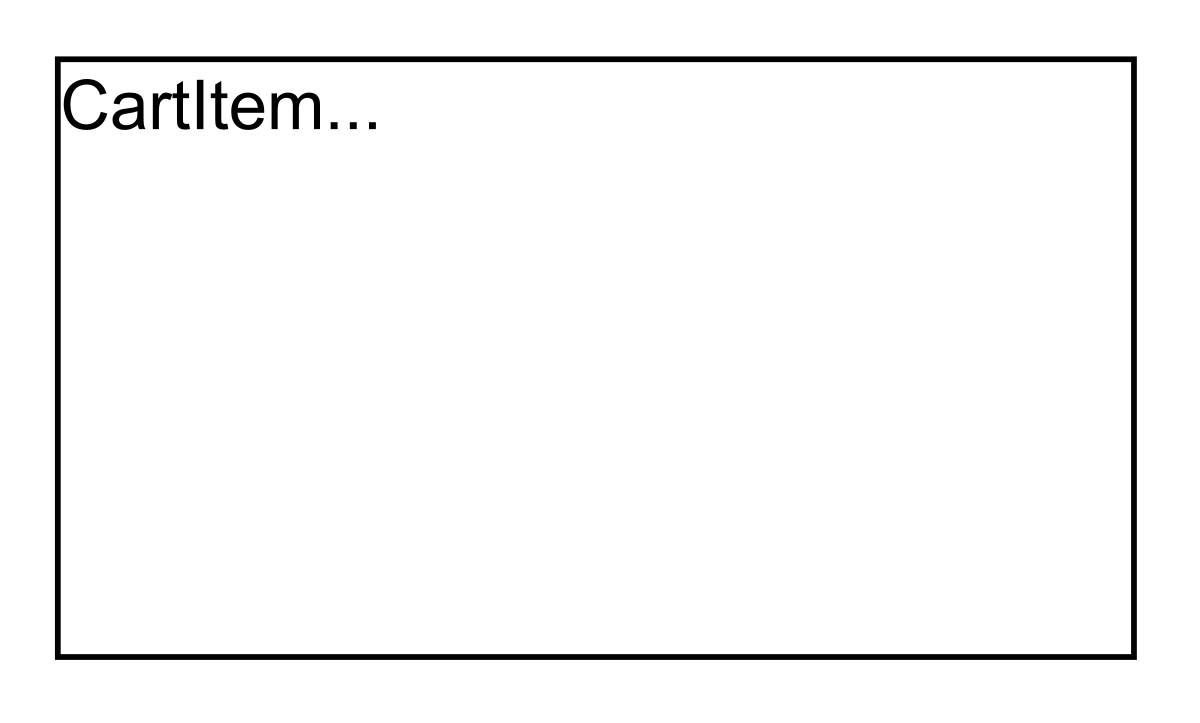
\includegraphics[width=0.5\textwidth]{Images/chapter_19/section_6113026015232000/6424338407227392.png}
 \caption{The class diagram of the CartItem class}
\end{figure}

\textbf{R4:} An authenticated user should be able to add, remove, or modify product items in their shopping cart. Then, the authenticated user can check out and buy the items.

\subsubsection{Shopping cart}\label{AYW_WK3f7xGe67F5RCYUE}
\\
The \texttt{ShoppingCart} class contains the list of cart items, upon which actions such as adding items to the cart, removing items from the cart, and accessing all cart items can be performed.

\begin{figure}[htbp]
 \centering
 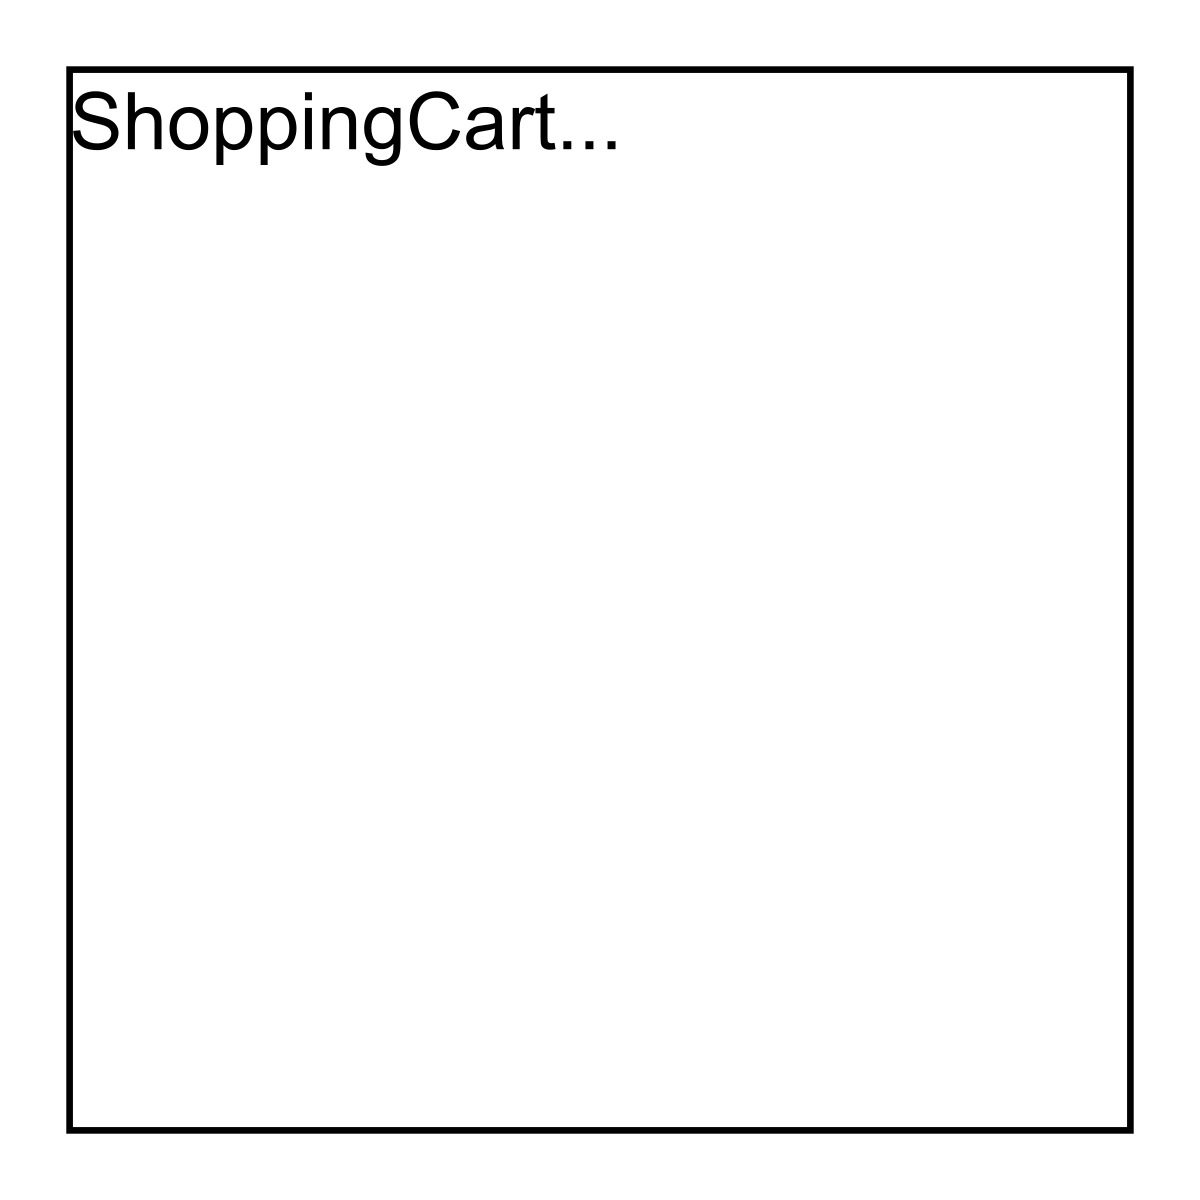
\includegraphics[width=0.5\textwidth]{Images/chapter_19/section_6113026015232000/4700322067775488.png}
 \caption{The class diagram of the ShoppingCart class}
\end{figure}

\textbf{R4:} An authenticated user should be able to add, remove, or modify product items in their shopping cart. Then, the authenticated user can check out and buy the items.

\subsubsection{Order}\label{Xm2TTi0EchNsNpHsWwOpD}
\\
The \texttt{Order} class refers to a particular customer's order and tracks its status, including the option of sending the order for shipment. It is also used to make the payment.

\begin{figure}[htbp]
 \centering
 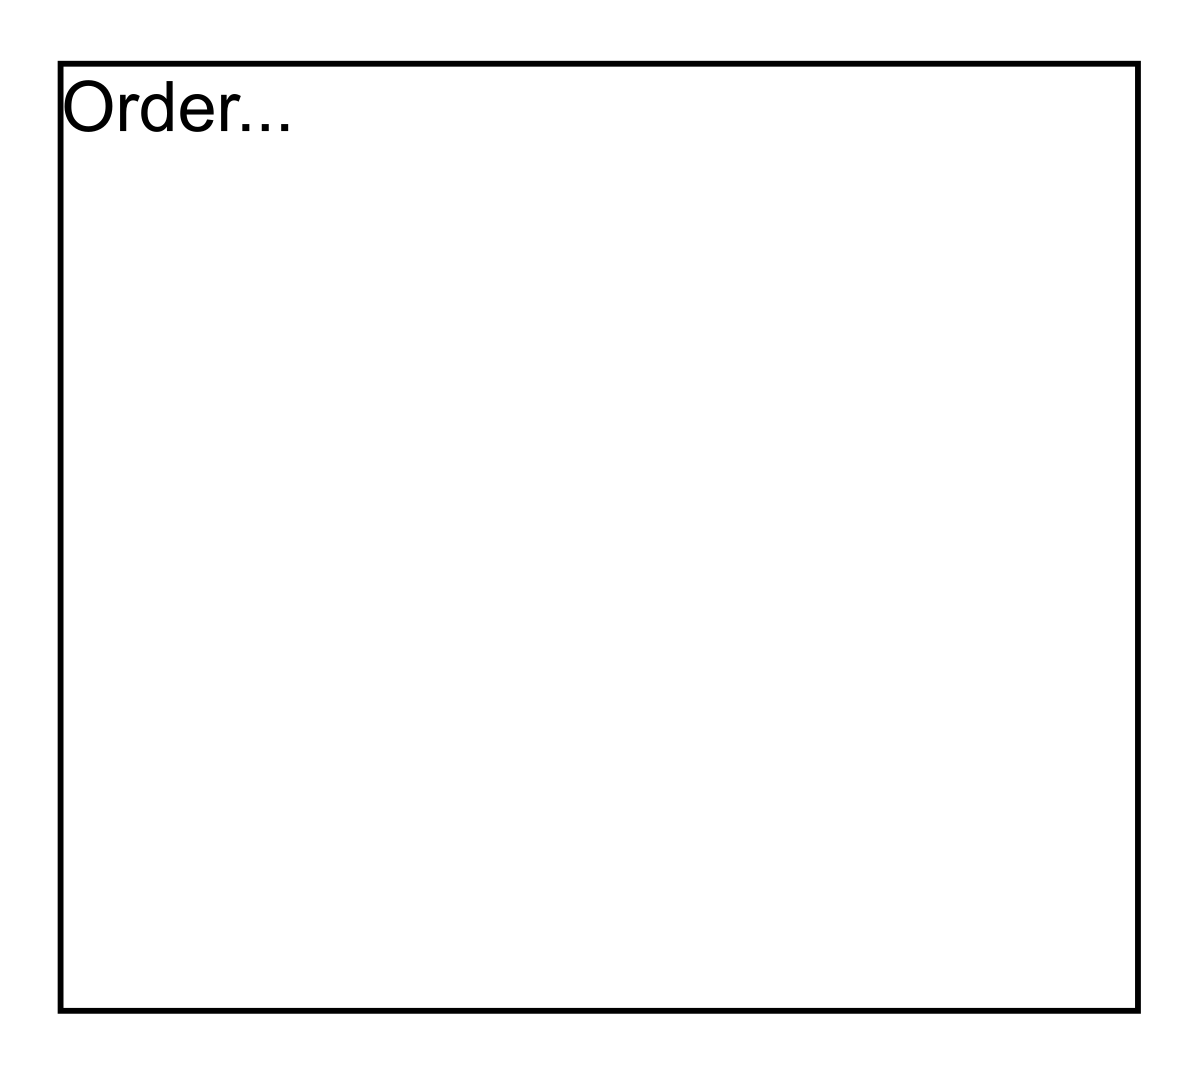
\includegraphics[width=0.5\textwidth]{Images/chapter_19/section_6113026015232000/6224714073505792.png}
 \caption{The class diagram of the Order class}
\end{figure}

\textbf{R7:} An order can be canceled only if it hasn't been shipped.

\subsubsection{Shipment}\label{Q8X82OBjryrT6pFOc8t3M}
\\
The \texttt{Shipment} class tracks the order's date, estimated arrival time, and shipment method. It will also be used to track the shipment status.

\begin{figure}[htbp]
 \centering
 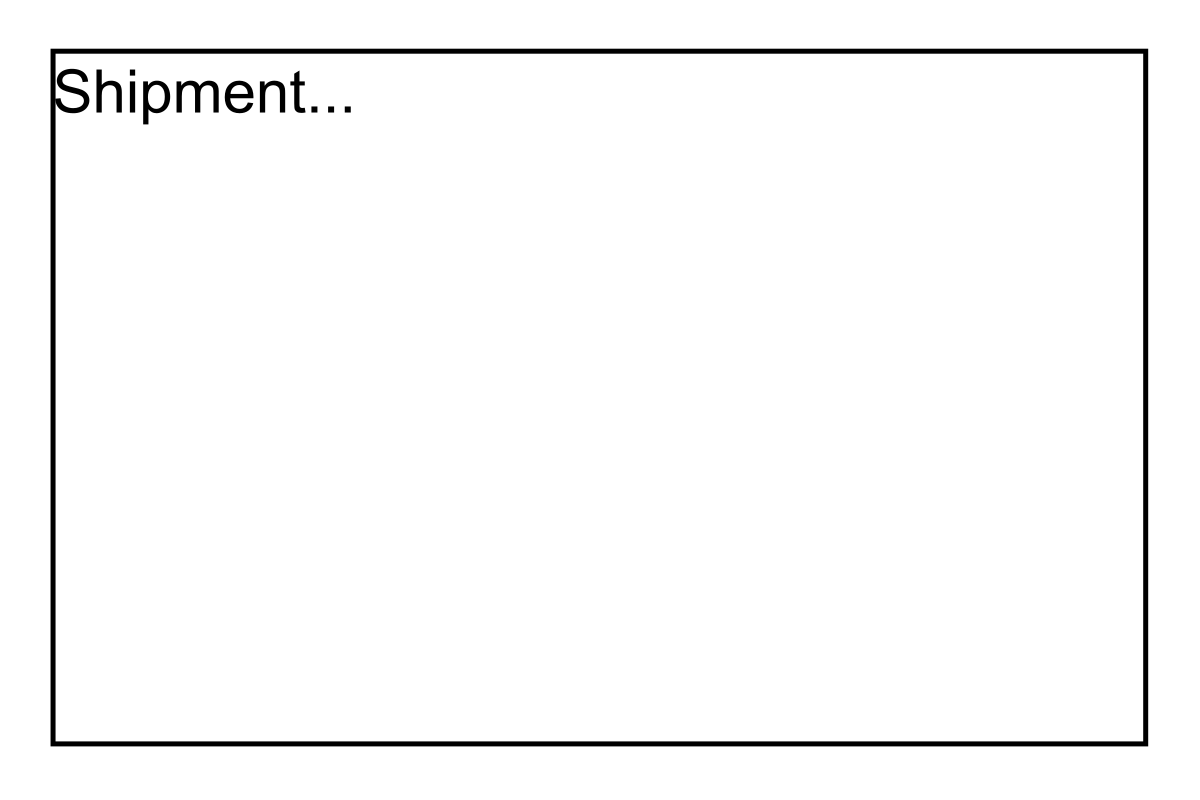
\includegraphics[width=0.5\textwidth]{Images/chapter_19/section_6113026015232000/4659335169703936.png}
 \caption{The class diagram of the Shipment class}
\end{figure}

\textbf{R9:} Shipment can be tracked to see the current status and the estimated arrival time for the order.

\subsubsection{Payment}\label{spPUwOm3kRzPiqkKehu98-2}
\\
The \texttt{Payment} class will have three child classes: \texttt{CreditCard}, \texttt{ElectronicBankTransfer}, and \texttt{Cash}, as these are the three payment methods available to a customer on Amazon.

\begin{figure}[htbp]
 \centering
 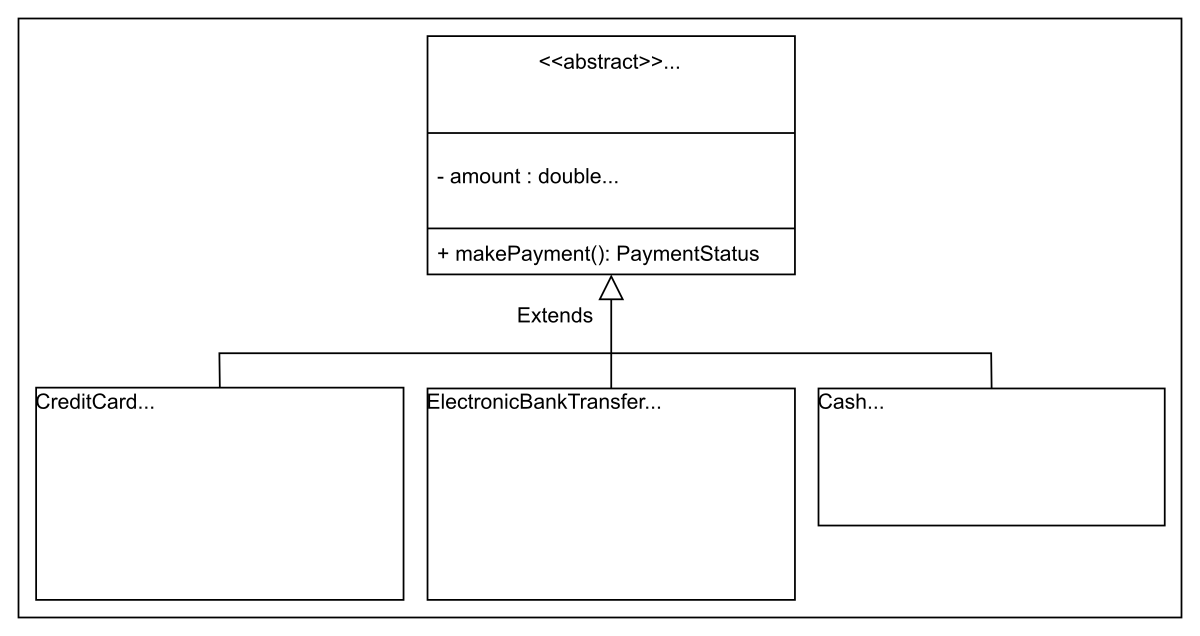
\includegraphics[width=0.5\textwidth]{Images/chapter_19/section_6113026015232000/5544234359586816.png}
 \caption{The class diagram of Payment and its child classes}
\end{figure}

\textbf{R6:} Payment can be made through credit cards, electronic bank transfers, or cash on delivery.

\subsubsection{Notification}\label{X3l4JnyP1sDlmkwtvLp9K}
\\
The \texttt{Notification} class is responsible for sending order and shipment notifications to customers shown below in the class diagram:
\begin{quote}
\textbf{Note:} Since the \texttt{Notification} class can be extended by adding various other options, we will implement it as an abstract class.
\end{quote}

\begin{figure}[htbp]
 \centering
 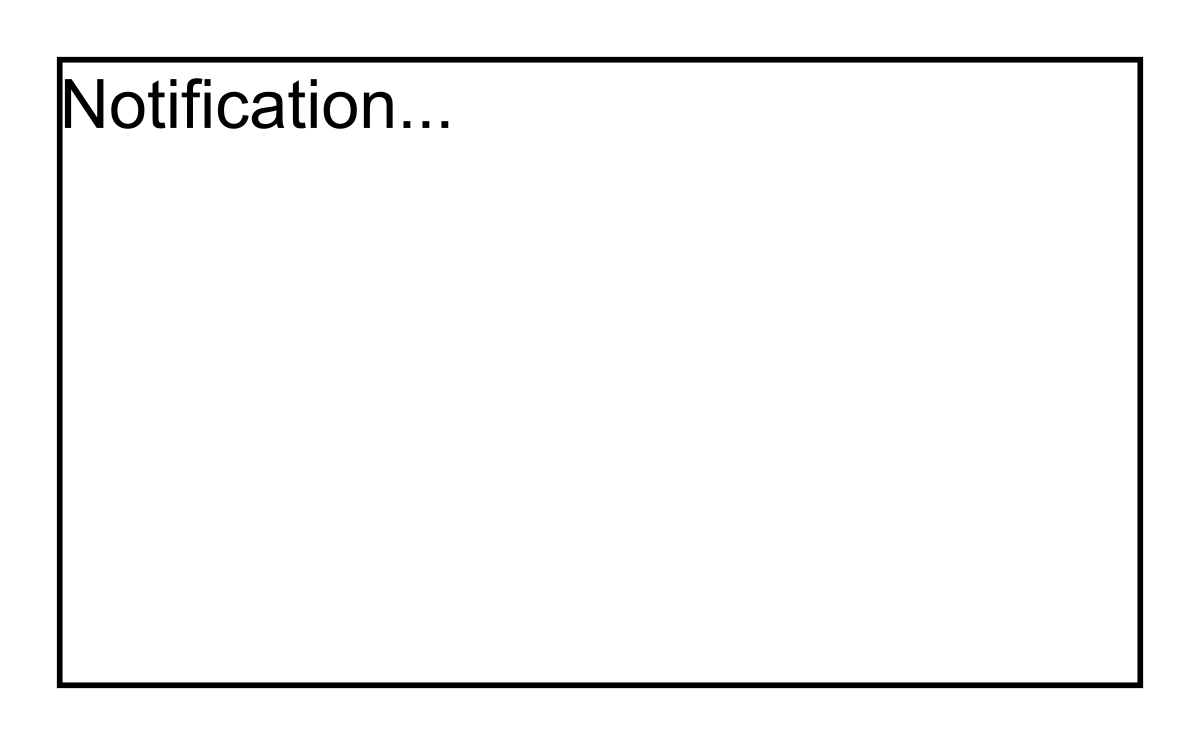
\includegraphics[width=0.5\textwidth]{Images/chapter_19/section_6113026015232000/5216348735930368.png}
 \caption{The class diagram of Notification and its child classes}
\end{figure}

\textbf{R8:} Notifications are sent whenever there is a change in the order or shipping status.

\subsubsection{Enumerations}\label{spPUwOm3kRzPiqkKehu98-3}
\\
The following is the list of enumerations required in Amazon:

\begin{itemize}
\item
\protect\phantomsection\label{9Q_NzedtwTRjX1cnD8dbF}
\texttt{AccountStatus}\textbf{:} The account status tells about the user account status, whether it is active, inactive, or blocked.
\item
\protect\phantomsection\label{gRJhV4ajrt7KuBbOFFRbw}
\texttt{PaymentStatus}\textbf{:} The payment status tells about the user account status, whether it is confirmed, declined, pending, or refunded.
\item
\protect\phantomsection\label{SmoZW2Hi2AC0TS8Pf7zdf}
\texttt{OrderStatus}\textbf{:} The order status describes the status of a particular order of a customer, whether it is unshipped, pending, shipped, confirmed, or canceled.hipped, confirmed, or canceled.
\item
\protect\phantomsection\label{5yaKAiF7T7rRjkC9Vu5OO}
\texttt{ShipmentStatus}\textbf{:} The shipment status tells us about the status of an order's shipment, whether it is in a pending state, shipped state, delivered state, or on hold.
\end{itemize}

\begin{figure}[htbp]
 \centering
 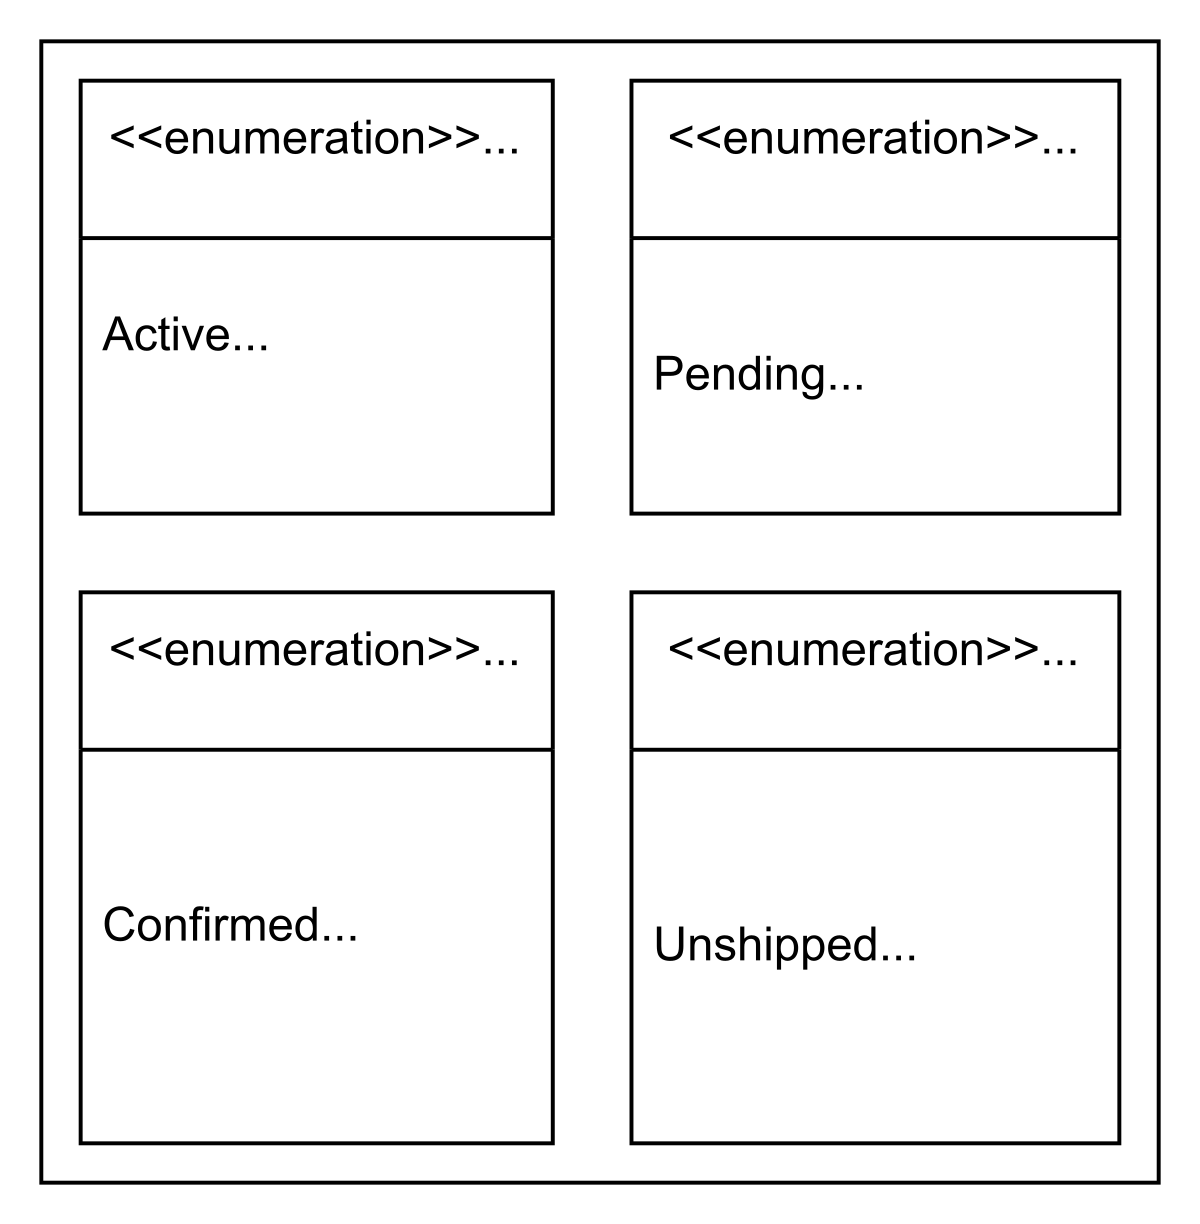
\includegraphics[width=0.5\textwidth]{Images/chapter_19/section_6113026015232000/5951528524185600.png}
 \caption{Enums in Amazon }
\end{figure}

\subsubsection{Custom data type}\label{spPUwOm3kRzPiqkKehu98-4}
\\
To store a customer's location, we must create a custom data type, \texttt{Address}.

\begin{figure}[htbp]
 \centering
 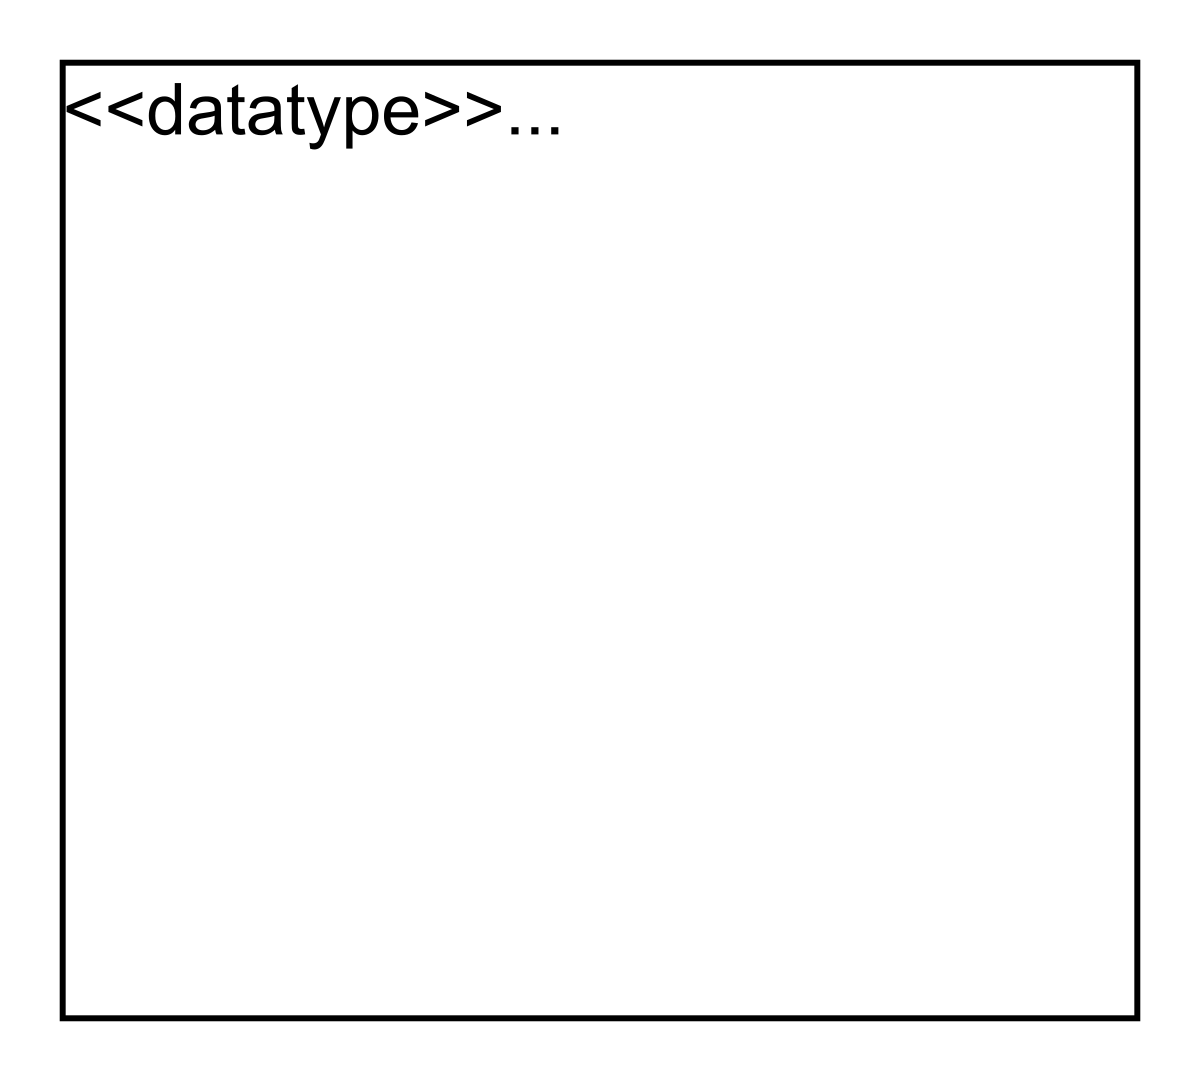
\includegraphics[width=0.5\textwidth]{Images/chapter_19/section_6113026015232000/5542782343970816.png}
 \caption{The class diagram of the Address custom data type}
\end{figure}

\subsection{Relationship between the classes}\label{spPUwOm3kRzPiqkKehu98-5}
\\
We'll discuss the relationships between the classes defined in our Amazon shopping system above.

\subsubsection{Association}\label{dvpKqdTP6PTEIlYOo1pIm}
\\
The class diagram has the following association relationships:

\begin{itemize}
\item
\protect\phantomsection\label{CKBgjmLGwQQRFbHyfmoJ_}
The \texttt{Notification} class has a \emph{one-way association} with \texttt{Shipment} and \texttt{Order}.
\item
\protect\phantomsection\label{FxcL5F4u9Mecqrx668MrD}
The \texttt{Product} class has a \emph{two-way association} with \texttt{Account} and \texttt{CartItem} and a \emph{one-way association} with \texttt{ProductCategory} and \texttt{ProductReview}.
\item
\protect\phantomsection\label{tudAGCgzOAJ3YA0mkqaCu}
The \texttt{ShoppingCart} class has a \emph{two-way association} with \texttt{CartItem}.
\item
\protect\phantomsection\label{Xo3u09JpK3RNiUPLAXLyv}
The \texttt{Order} class has a \emph{two-way association} with \texttt{Payment} and a \emph{one-way association} with \texttt{Shipment} and \texttt{ShoppingCart}.
\end{itemize}

\begin{figure}[htbp]
 \centering
 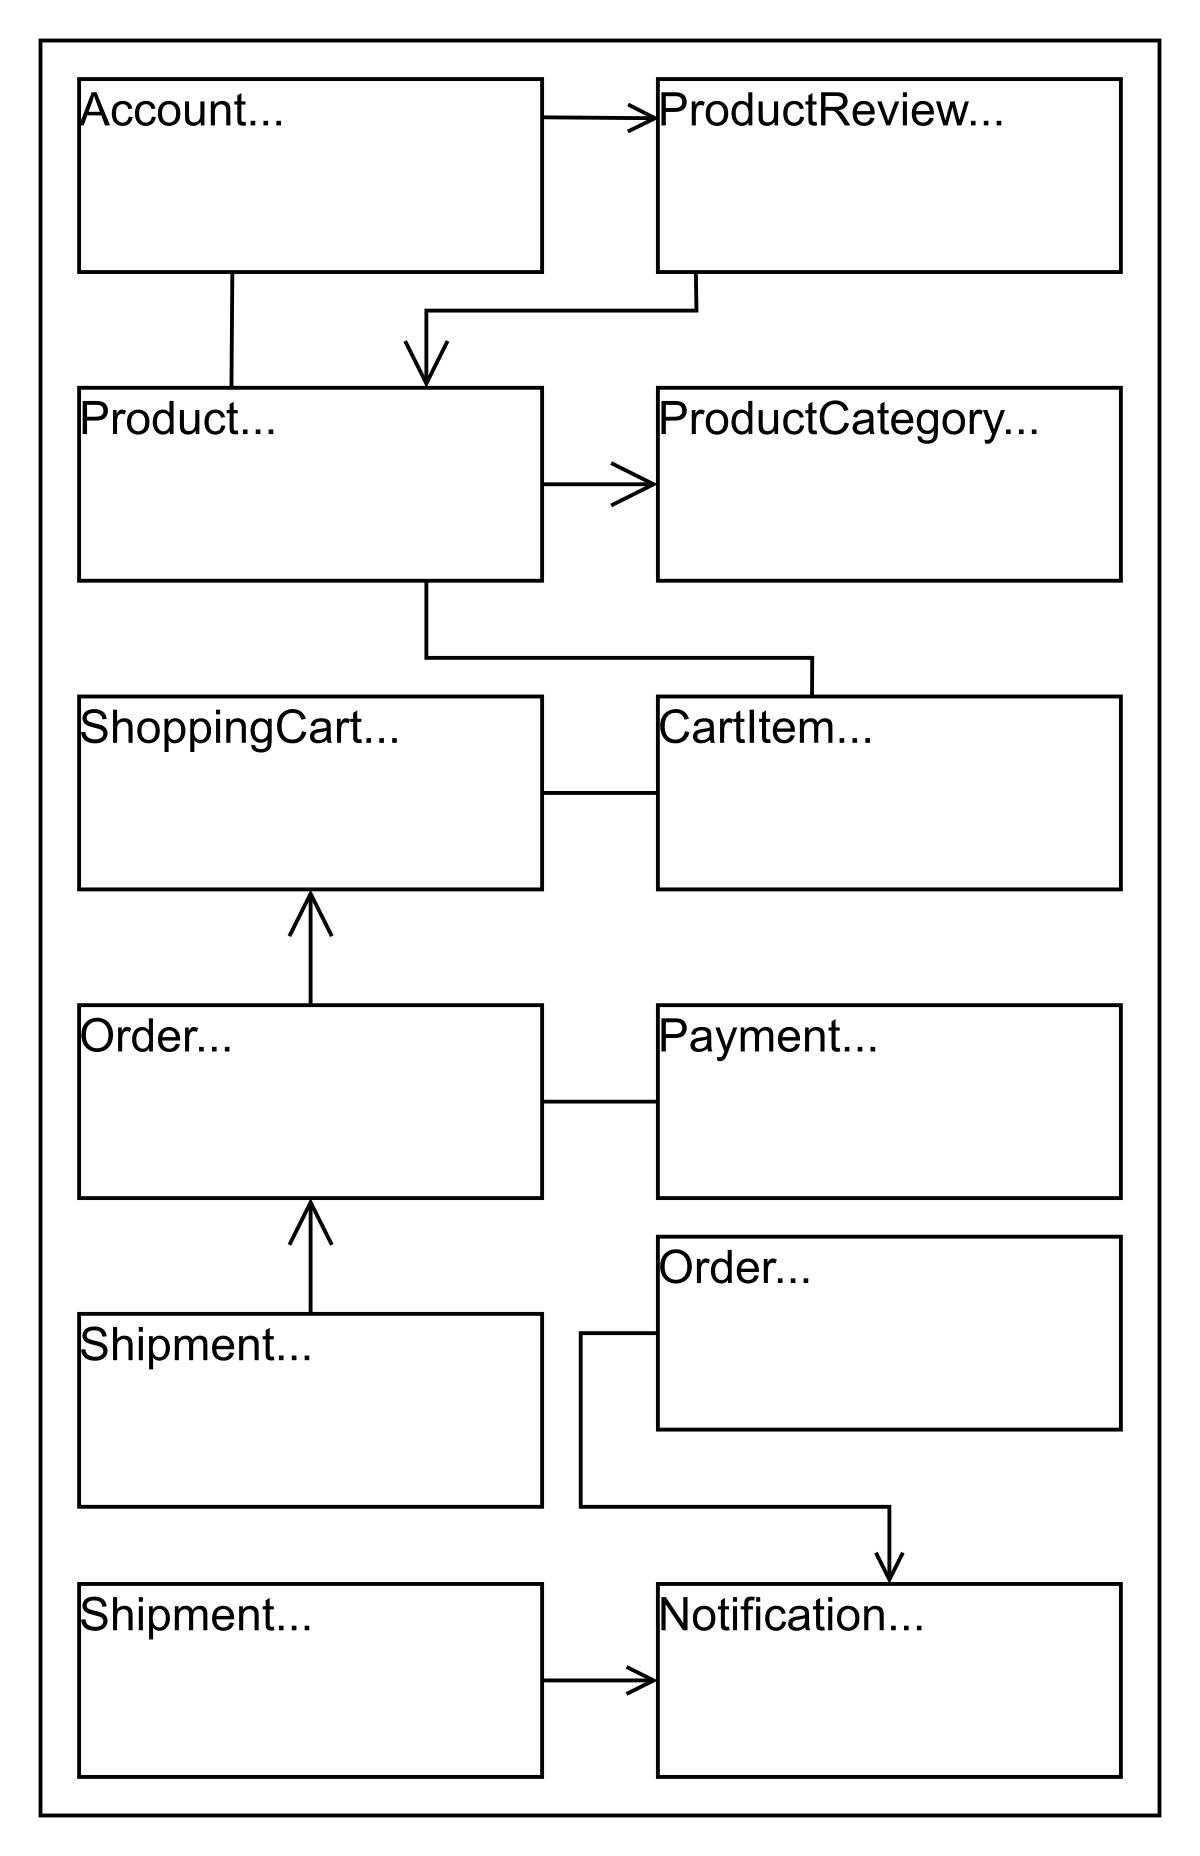
\includegraphics[width=0.5\textwidth]{Images/chapter_19/section_6113026015232000/5069576445231104.png}
 \caption{The association relationship between classes}
\end{figure}

\subsubsection{Composition}\label{sRPF-Fg57bssQyLcVzkNe}
\\
The class diagram has the following composition relationships:

\begin{itemize}
\item
\protect\phantomsection\label{ytSCVmLz2qOgE8WArgHWz}
The \texttt{Account} class is composed of the CreditCard\ and \texttt{ElectronicBankTransfer}.
\item
\protect\phantomsection\label{T2D1tMV0uHrtqHM-rpGn4}
The \texttt{Admin} and \texttt{AuthenticatedUser} classes are composed of \texttt{Account}.
\item
\protect\phantomsection\label{TmYfp1XGwg4VkpF9oF7cL}
The \texttt{AuthenticatedUser} class is composed of the \texttt{Order} class.
\item
\protect\phantomsection\label{21kVxPLewnqA9oeVOGRJG}
The \texttt{Customer} class is composed of the \texttt{ShoppingCart} class.
\end{itemize}

\begin{figure}[htbp]
 \centering
 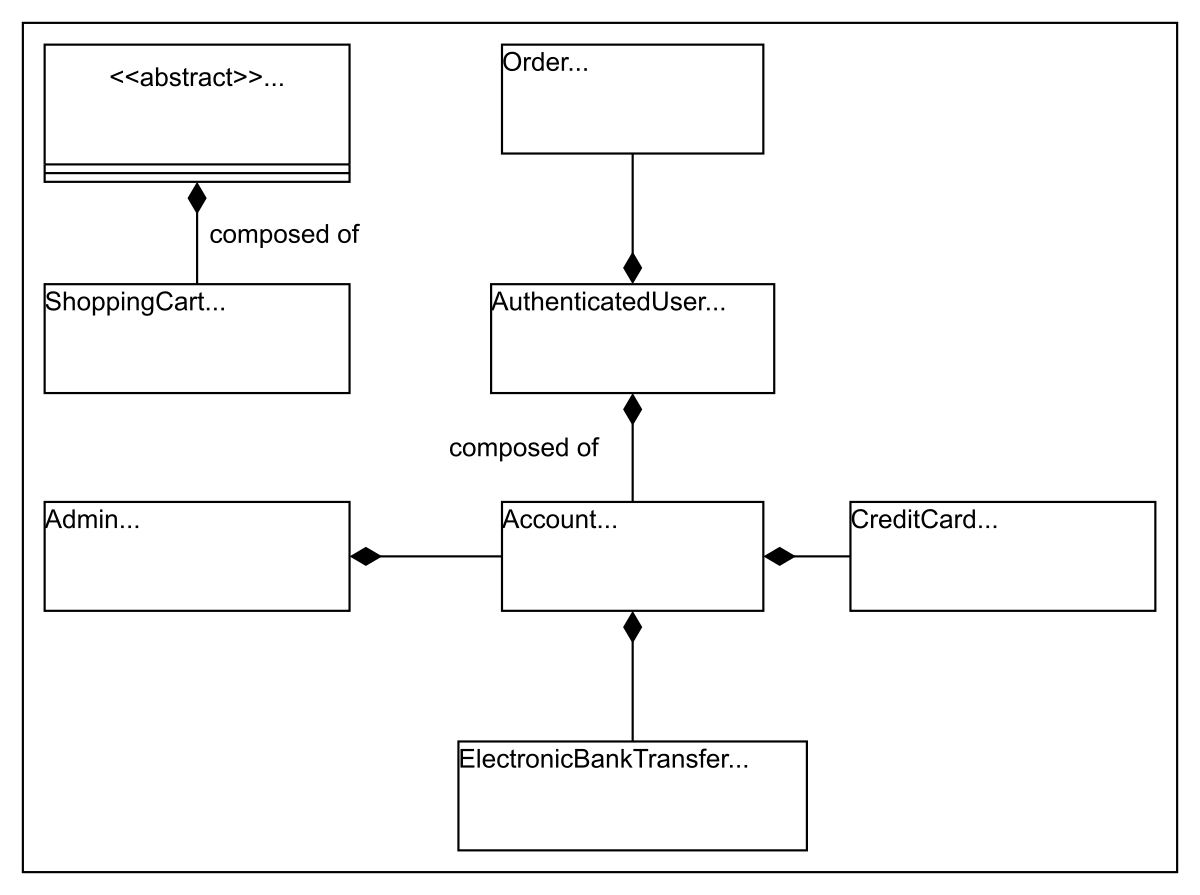
\includegraphics[width=0.5\textwidth]{Images/chapter_19/section_6113026015232000/4704311480025088.png}
 \caption{The composition relationship between classes}
\end{figure}

\subsubsection{Aggregation}\label{spPUwOm3kRzPiqkKehu98-6}
\\
The following class show an aggregation relationship:

\begin{itemize}
\item
\protect\phantomsection\label{4ALOSkR__mWCAxp25KAF-}
The \texttt{Product} class has an aggregation relation with the Search class.
\end{itemize}

\begin{figure}[htbp]
 \centering
 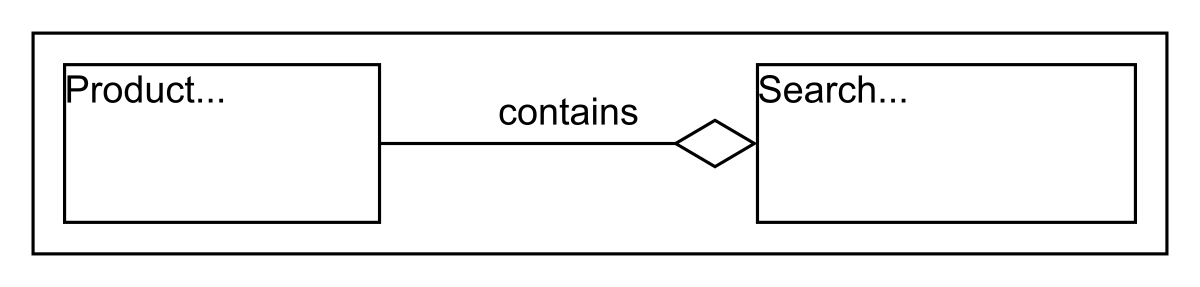
\includegraphics[width=0.5\textwidth]{Images/chapter_19/section_6113026015232000/5915817920036864.png}
 \caption{The aggregation relationship between classes}
\end{figure}

\subsubsection{Inheritance}\label{spPUwOm3kRzPiqkKehu98-7}
\\
The following classes show an inheritance relationship:

\begin{itemize}
\item
\protect\phantomsection\label{OGb42QBkYAJ3_FBBVFKjh}
Both \texttt{Guest} and \texttt{AuthenticatedUser} extend the \texttt{Customer} class.
\item
\protect\phantomsection\label{KxxaeYiRvuMGLPKZn6sPp}
Subclasses \texttt{Cash}, \texttt{ElectronicBankTransfer}, and \texttt{CreditCard} extend the \texttt{Payment} class.
\end{itemize}
\begin{quote}
\textbf{Note:} The component section above has already discussed the inheritance relationship between classes.
\end{quote}
\subsection{Class diagram of Amazon}\label{ZxkKBEk4wlhTrTa_fE-oh}
\\
This section outlines the multiplicity (cardinality) relationships between the main classes in our Amazon online shopping system. We explain the allowed number of instances on each side for each relationship and the real-world or design rationale behind the connection. Understanding these relationships is key to modeling how different entities interact and collaborate to support key workflows in the system.

\begin{table}[h!]
\centering
\begin{tabular}{|p{3.5cm}|p{3.5cm}|p{3cm}|p{6.5cm}|}
\hline
\textbf{Source} & \textbf{Target} & \textbf{Multiplicity} & \textbf{Reason} \\
\hline
Address & ProductCategory & 1--0..* & One Address can be associated with many ProductCategory objects. \\
\hline
ProductCategory & Product & 1--0..* & One ProductCategory can have many Products, but a Product belongs to exactly one ProductCategory. \\
\hline
Product & ProductReview & 1--0..* & One Product can have many ProductReview objects. \\
\hline
ProductReview & AuthenticatedUser & 1--1 & One ProductReview is written by one AuthenticatedUser. \\
\hline
Admin & Account & 1--0..* & One Admin can manage multiple Account objects. \\
\hline
Account & Order & 1--0..* & One Account can place many Order objects. \\
\hline
Order & Shipment & 1--0..* & One Order can be associated with many Shipment objects. \\
\hline
Order & PaymentStatus & 1--1 & One Order has exactly one PaymentStatus object. \\
\hline
ProductCategory & Admin & 1--1 & One ProductCategory is managed by one Admin. \\
\hline
ShoppingCart & Product & 1--0..* & One ShoppingCart can contain multiple Product objects. \\
\hline
Guest & Product & 1--0..* & One Guest can search many Product objects. \\
\hline
Search & Product & 1--0..* & One Search operation can return multiple Product objects. \\
\hline
AuthenticatedUser & ShoppingCart & 1--1 & One AuthenticatedUser can have exactly one ShoppingCart. \\
\hline
ShoppingCart & Order & 1--1 & One ShoppingCart is associated with exactly one Order. \\
\hline
\end{tabular}
\caption{Entity Relationships and Multiplicities in an E-Commerce System}
\label{tab:ecommerce_entity_relationships}
\end{table}


Here's the complete class diagram for Amazon:

\begin{figure}[htbp]
 \centering
 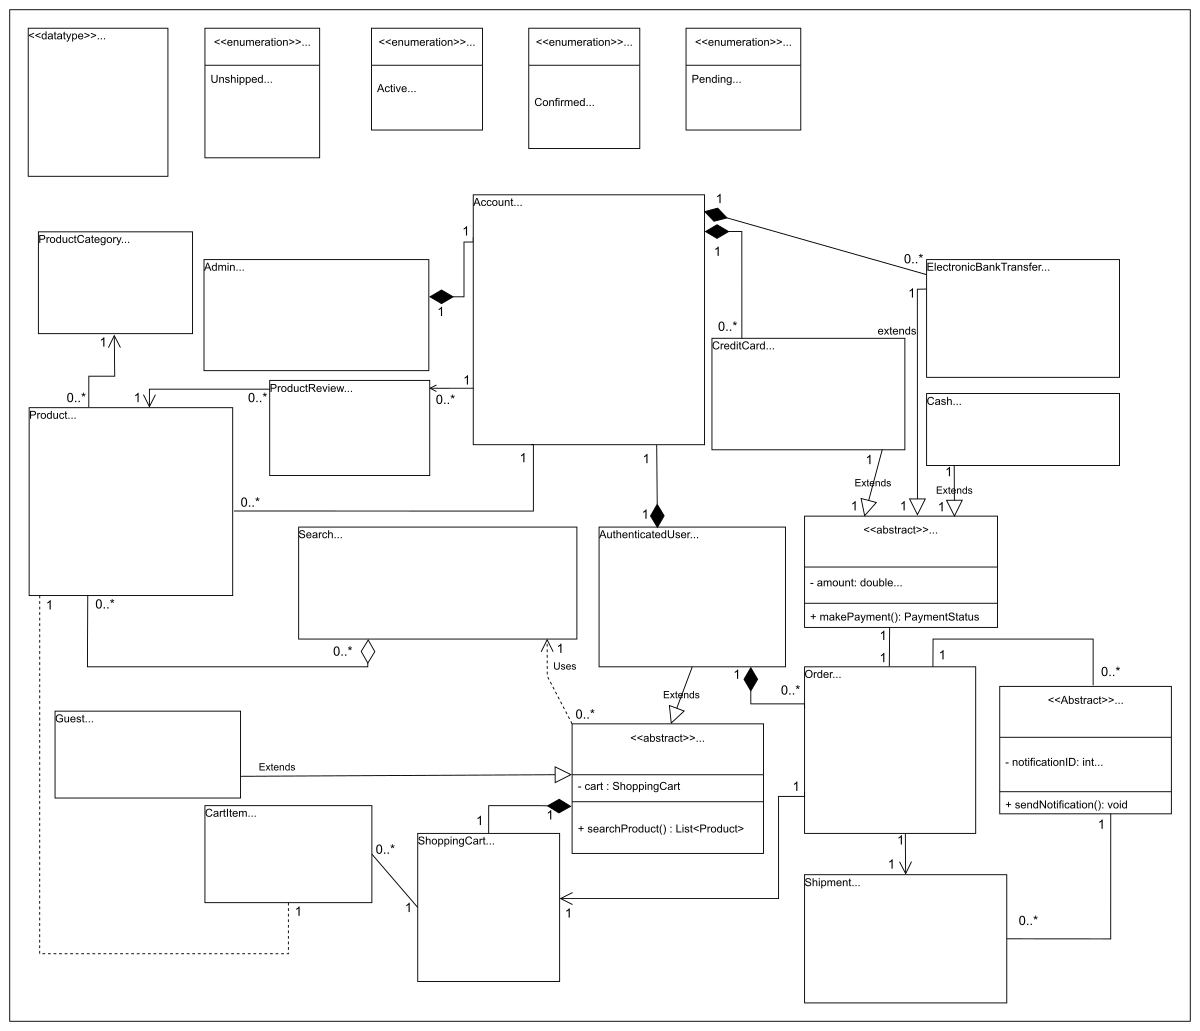
\includegraphics[width=0.5\textwidth]{Images/chapter_19/section_6113026015232000/6617945210748928.png}
 \caption{The class diagram of Amazon}
\end{figure}

\subsection{Design pattern}\label{oq4x6Ln5i_JUFb9fOYMUm}
\\
The following design patterns have been used in the class diagram:

\begin{itemize}
\item
We know that the system needs to create different types of accounts, such as \texttt{AuthenticatedUser} and \texttt{Guest} accounts. To model this behavior, we can use the Factory Method pattern.
\item
We know that a restaurant can accept different types of payments, such as \texttt{Cash}, \texttt{CreditCards}, and \texttt{ElectronicBankTransfers}. To model this behavior, we can use the Strategy pattern.
\item
We know that a \texttt{ShoppingCart} can contain multiple \texttt{Product} objects, and a \texttt{ProductCategory} can also contain multiple \texttt{Product} objects. To model this behavior, we can use the Composite pattern.
\item
When an order's status changes, we know that customers need to be notified. To model this behavior, we can use the Observer pattern.
\item
\protect\phantomsection\label{Fm-1AC8bAKyiFCmB5W67u}
We know that various actions need to be performed on the \texttt{Order} and \texttt{ShoppingCart}, such as \texttt{placeOrder(),} \texttt{makePayment(),} and \texttt{addProduct().} To model this behavior, we can use the Command pattern.
\end{itemize}

\subsection{AI-powered trainer}\label{nPXcnxneRTDYRoEqmhMZr}
\\
At this stage, everything should be clear. If you encounter any confusion or ambiguity, feel free to utilize the interactive AI-enabled widget below to seek clarification. This tool is designed to help you strengthen your understanding of the concepts.

\begin{figure}[htbp]
 \centering
 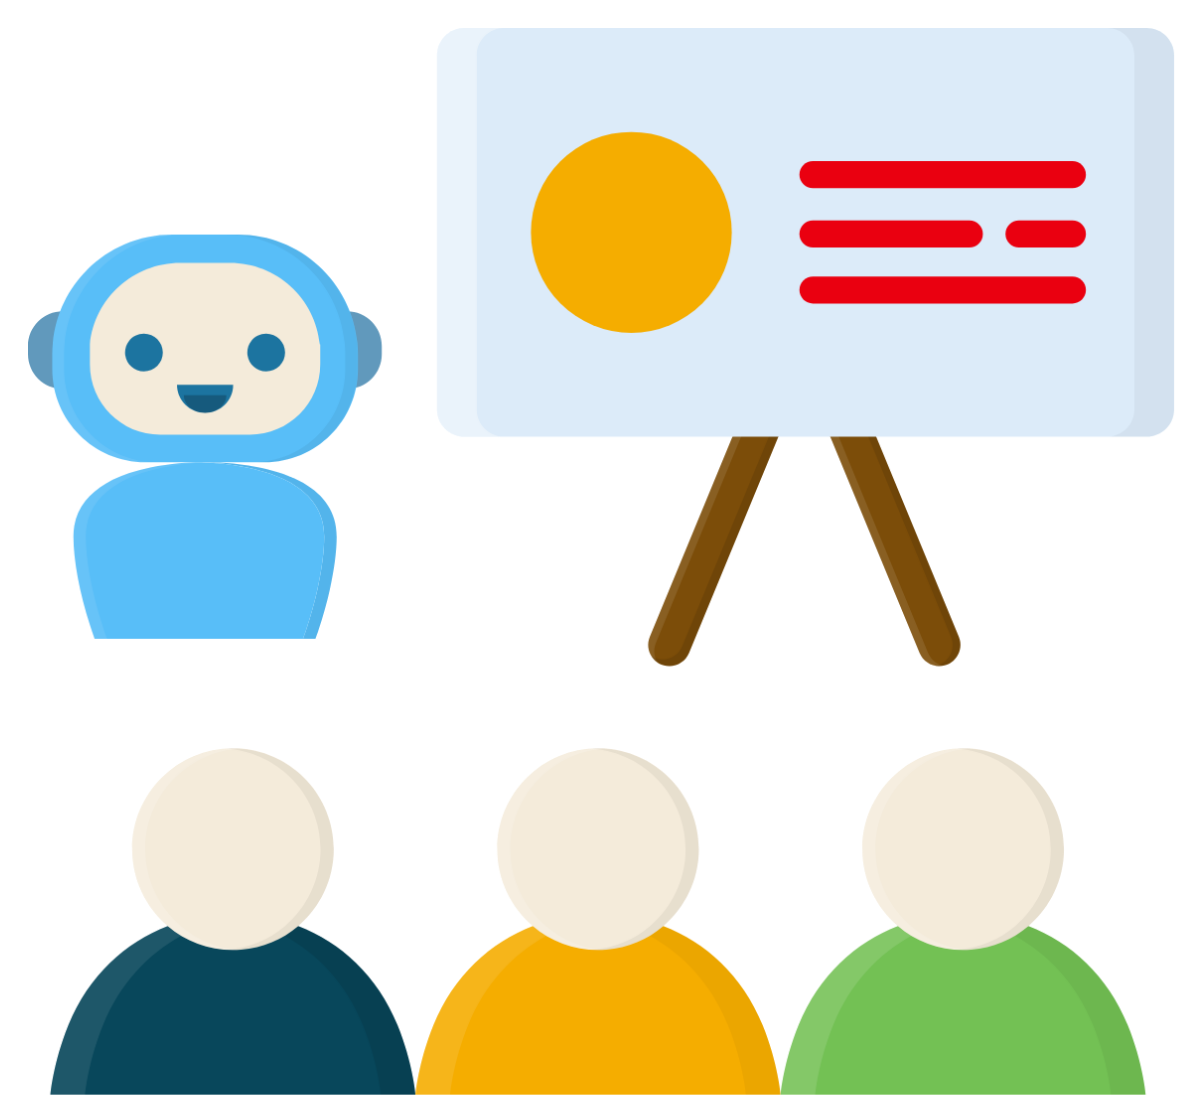
\includegraphics[width=0.15\textwidth]{Images/chapter_19/section_6113026015232000/5779861464285184.png}
 
\end{figure}

\subsection{Additional requirements}\label{n-5b0Ee1x4DUTyc2TS94H}
\\
The interviewer can introduce some additional requirements in the Amazon shopping system, or they can ask some follow-up questions. Let 's see some examples of additional requirements:
\\
\textbf{Wish list:} Only authenticated users can have a wish list, and they can add products to their wish list. Wish list items can be moved to the user's shopping cart. The \texttt{Wishlist} class has a two-way association with the \texttt{Product} class, as a wish list can contain multiple products, and products can belong to multiple wish lists, while it has an aggregation relationship with the \texttt{User} class, as a user can have a wish list, and a wish list cannot exist without a user.

\begin{figure}[htbp]
 \centering
 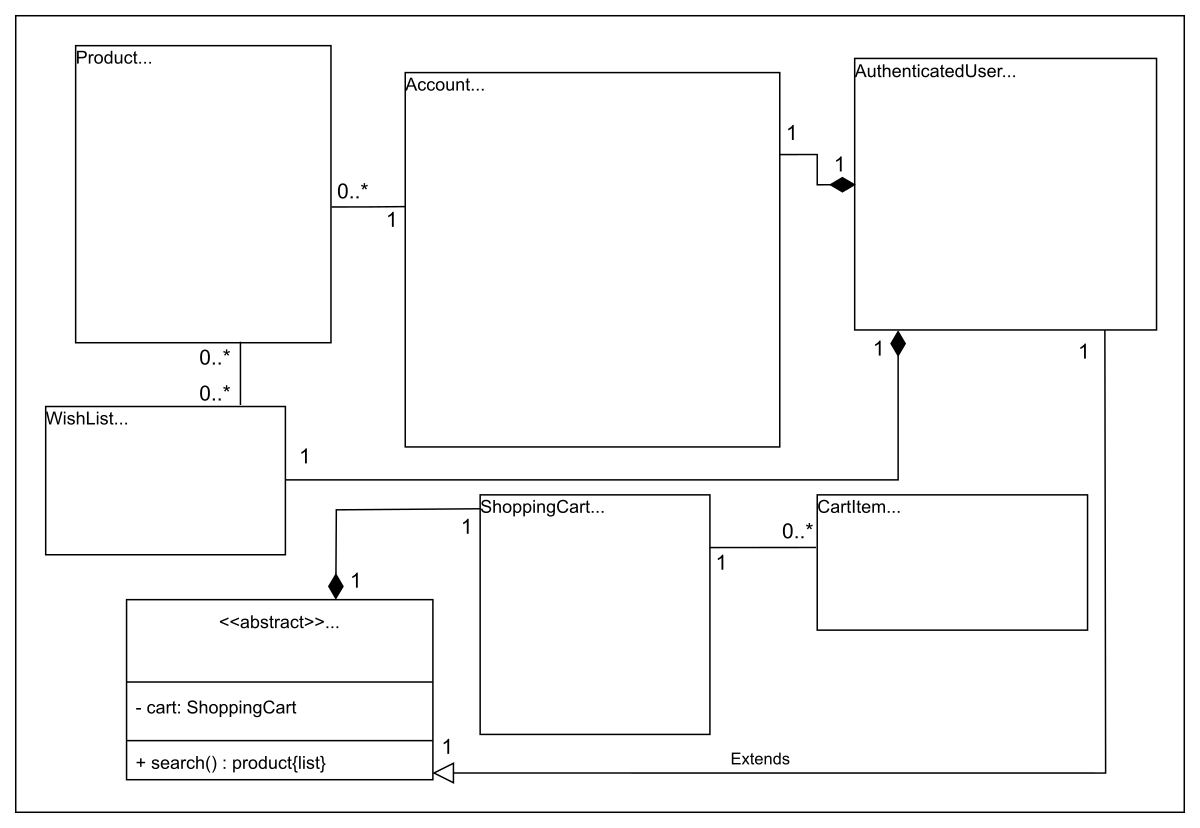
\includegraphics[width=0.5\textwidth]{Images/chapter_19/section_6113026015232000/5470244876189696.png}
 \caption{ Adding Wishlist functionality}
\end{figure}

\textbf{Discount:} A discount will be applied to the payment depending on special events such as Christmas, Black Friday, etc. The \texttt{Payment} class has a one-way association with the \texttt{Discount} class, as a payment can receive a discount, but the discount is linked to the payment and does not exist independently.

\begin{figure}[htbp]
 \centering
 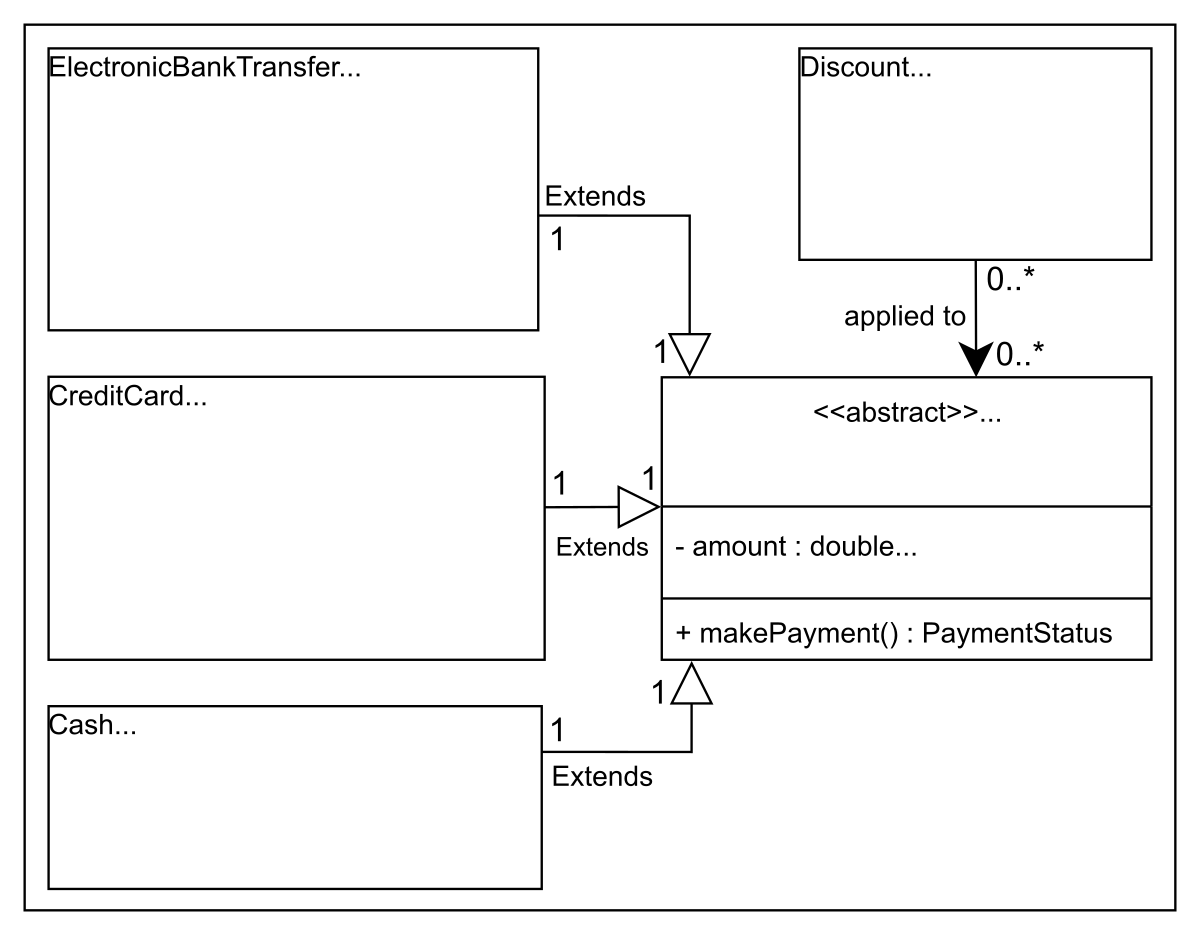
\includegraphics[width=0.5\textwidth]{Images/chapter_19/section_6113026015232000/5414692678664192.png}
 \caption{Relationship between the Discount class with the Payment class}
\end{figure}

We've completed the class diagram of the Amazon shopping system according to the requirements. Now , let's design the sequence diagram of the Amazon shopping system in the next lesson.

% End of section content